\documentclass{beamer}

\mode<presentation> {
	\usetheme{Berkeley}
}

\usepackage{graphicx}
\usepackage{booktabs}
\usepackage[english]{babel}

\title[Sprint Review]{ROW5 Sprint 3 Review}

\author{ROW Team 5}
\institute[HvA]
{
	Amsterdam University of Applied Sciences \\
	\textit{https://rescueonwheels.github.io/}
}
\date{December 3, 2018}

\begin{document}

\begin{frame}
\titlepage % Print the title page as the first slide
\end{frame}

\section{Introduction}
\begin{frame}{Introduction}
    \begin{center}
        \begin{tabular}{c|c}
             Christiaan van Arum    & Developer \\
             \hline
             Rapha\"{e}l Bunck & Scrum Master \\
             \hline
             Nino van Galen & Developer \\
             \hline
             Martijn Vegter & Product Owner
         \end{tabular}
    \end{center}
\end{frame}

\begin{frame}
\frametitle{Overview} % Table of contents slide, comment this block out to remove it
\tableofcontents % Throughout your presentation, if you choose to use \section{} and \subsection{} commands, these will automatically be printed on this slide as an overview of your presentation
\end{frame}

\section{Sprint goal}
\begin{frame}{Sprint Goal}
\normalsize{\centerline{"Focus on autonomous behavior."}}
\end{frame}

\section{Our progress}
\begin{frame}{Our Progress}
    \begin{itemize}
    \item Virtual Reality is, finally, working
    \item Improved communication, software and hardware
    \item Improved auto-stop functionality
    \item Updated documentation
    \item Proof of Concept: Epicenter
\end{itemize}
\end{frame}

\section{Process}
\begin{frame}{Process}
    \begin{itemize}
        \item What went well?
        \item Problems we ran into
        \item How we solved those problems
    \end{itemize}
\end{frame}

\section{Burndown}
\begin{frame}{Burndown}
    \begin{center}
      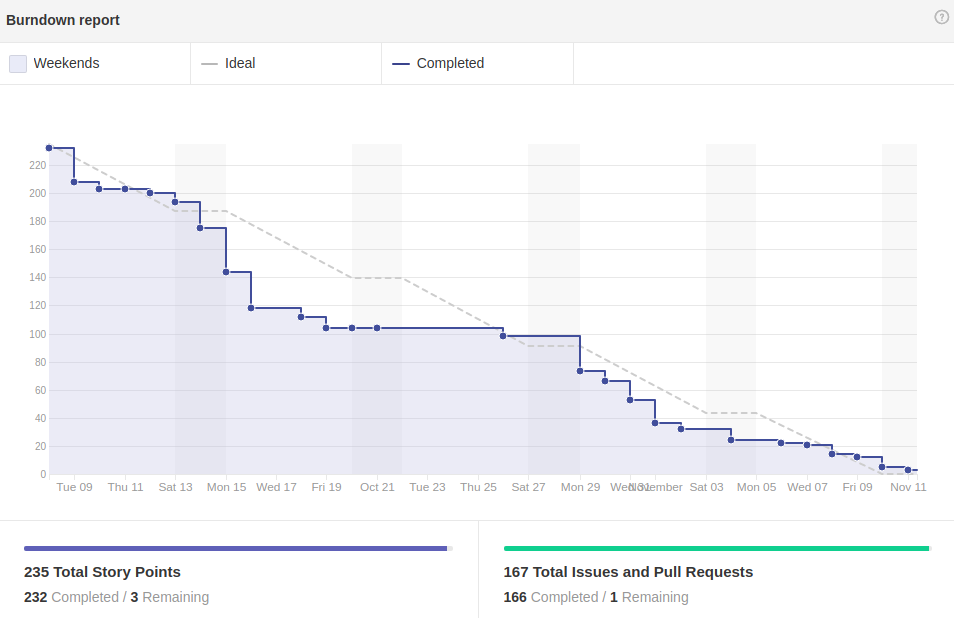
\includegraphics[scale=1.25]{images/burndown.png}
    \end{center}
\end{frame}

\section{Coaching}
\begin{frame}
\Huge{\centerline{We had coaching}}
\end{frame}

\section{What's Next? }
\begin{frame}{What's next?}
    \begin{itemize}
        \item Improve VR app
        \item Improve documentation
        \item Remove code related to mappping
    \end{itemize}
\end{frame}

\section{End}
\begin{frame}
\Huge{\centerline{The End}}
\end{frame}

\end{document}